% !TEX root = ../main.tex

\chapter{Introduction}
\section{The First Section}
Lorem ipsum dolor sit amet\cite{einstein,latexcompanion,knuthwebsite}, consectetur adipiscing elit. Sed aliquam elit at massa sodales, eu imperdiet ligula feugiat. Quisque nec eros sodales, pretium est sodales, iaculis lorem. Suspendisse in semper diam, nec mollis urna. Aliquam gravida lobortis ligula. Fusce pulvinar mi ipsum. Ut nibh turpis, auctor vitae interdum sit amet, fermentum non turpis. Praesent vel risus commodo, dapibus enim ac, maximus neque. Duis convallis, massa et cursus dapibus, leo erat mattis neque, ac interdum quam tortor sit amet justo. Morbi ac dui interdum, posuere risus a, pulvinar mi. Maecenas faucibus consequat suscipit. Maecenas lacinia sit amet tellus sed molestie. Suspendisse bibendum commodo dolor, vitae pulvinar lorem condimentum vitae. Sed molestie condimentum pharetra. Etiam viverra lobortis mi, a vehicula sem convallis id. Etiam gravida arcu et tellus scelerisque ultricies. Cras sed porta ipsum, sed consectetur lorem.

\begin{figure}[p]
    \centering
    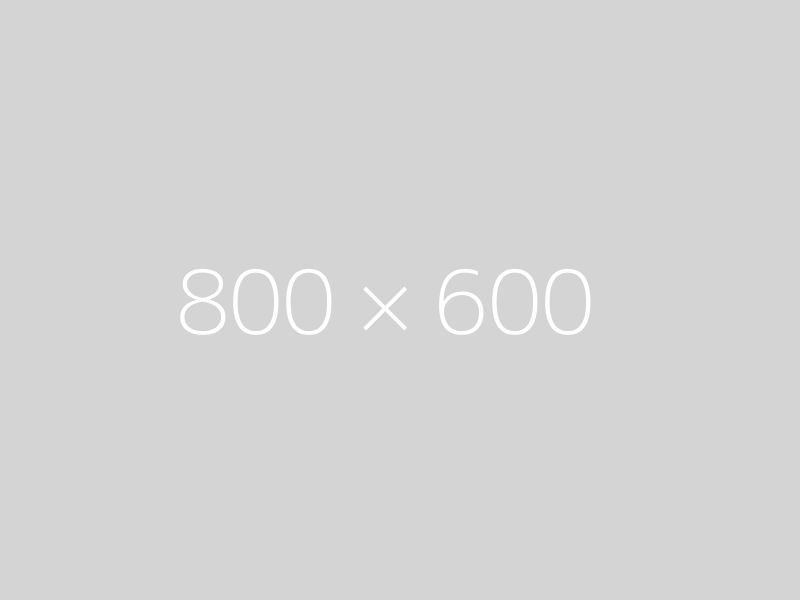
\includegraphics[width=\textwidth]{figures/placeholder.png}
    \caption[An example Figure 1.]{\textbf{An example Figure 1.} An example 800x600 figure, that should be displayed in a new page. If you don't like it, then check this web page for more information on the figure positioning: \href{https://www.overleaf.com/learn/latex/Positioning_of_Figures}{https://www.overleaf.com/learn/latex/Positioning\_of\_Figures}}
    \label{figlabel1}
\end{figure}

